% SS10 / Narxoz Research Methods. Proposed study + SYNTHETIC demonstration.
% Compiler: pdfLaTeX; citations: BibTeX (IEEEtran numeric style).
\documentclass[conference]{IEEEtran}
\usepackage[T1]{fontenc}
\usepackage[utf8]{inputenc}
\usepackage{lmodern}
\usepackage{amsmath,amssymb}
\usepackage{booktabs}
\usepackage{graphicx}
\usepackage{tikz}
\usetikzlibrary{arrows.meta,positioning,shapes.geometric}
\usepackage[hidelinks]{hyperref}
\usepackage{url}
\title{The Impact of Generative AI Tools on Employee Productivity and Work Quality in Knowledge-Based Office Tasks}
\author{
   \IEEEauthorblockN{Muratbek Ramazan}
   \IEEEauthorblockA{Narxoz University\\Almaty, Kazakhstan}
   \and
   \IEEEauthorblockN{Tasbolatkyzy Zhanerke}
   \IEEEauthorblockA{Narxoz University\\Almaty, Kazakhstan}
}
\begin{document}
\maketitle
\begin{abstract}
This paper presents a reproducible protocol for evaluating generative AI assistance in professional writing. We propose a randomized, counterbalanced crossover comparison using matched writing tasks, a fair no-AI baseline, completion-time measures, blinded quality scoring, and factual-evaluation rules. We describe a reproducible Python analysis pipeline and show synthetic examples for verification only. Four fictional participant pairs and 100 separate software-benchmark runs are used to test reporting, not to estimate workplace productivity. No participants have yet been recruited; thus, this manuscript reports a study design and software demonstration rather than empirical findings.
\end{abstract}
\begin{IEEEkeywords}
  generative AI, knowledge work, experimental design, writing productivity, reproducibility, paired bootstrap
\end{IEEEkeywords}
\section{Introduction}\label{sec:introduction}
\subsection{Context and motivation}
Generative artificial intelligence (GenAI) tools increasingly support writing, information synthesis, and other knowledge-based office activities. Their effectiveness cannot be established from a software speed test alone: human completion time, output quality, and factual correctness are different outcomes. Previous empirical studies have reported productivity benefits in professional writing~\cite{noyExperimentalEvidenceProductivity2023} and customer-support work~\cite{brynjolfssonGenerativeAIWork2023}.

\subsection{Research gap}
Existing evidence concerns distinct occupations, task types, and intervention conditions. In particular, the potential advantage of AI assistance varies with task characteristics, and favorable average results do not guarantee correct performance on every assignment~\cite{dellacquaNavigatingJaggedTechnological2026}. Automation and augmentation also raise different questions about the role of human oversight~\cite{raischArtificialIntelligenceManagement2021}. This motivates a local, reproducible protocol in which the no-AI condition remains a realistic human baseline and quality is checked alongside duration. We do not claim these cited studies establish an effect in our proposed sample.

\subsection{Research questions and contributions}
The primary research question is: \emph{Does allowing GenAI assistance reduce the time required to complete matched professional writing tasks?} The primary estimand is within-participant mean time saved. A secondary question asks whether quality and factual coverage are preserved. Exploratory work will examine task order and professional experience. Survey-based questions about AI adoption (RQ1) would require separate data and are not answered by the crossover alone.

This work makes the following \emph{methodological}, rather than empirical, contributions:
\begin{itemize}
  \item A fair within-participant AI/no-AI comparison with counterbalanced task and condition order;
  \item A prespecified analysis of completion time, blinded quality assessment, and factual correctness;
  \item An auditable synthetic-data implementation with validation, uncertainty calculations, and clearly separated software-performance instrumentation.
\end{itemize}

\subsection{Paper organization}
Section~\ref{sec:methodology} details the experimental protocol and estimands. Section~\ref{sec:demonstration} presents synthetic verification outputs. Section~\ref{sec:discussion} discusses limitations, reproducibility, and the work required for empirical conclusions.

\section{Methodology}\label{sec:methodology}
\subsection{Design and conditions}
We propose a randomized counterbalanced crossover with matched writing sets A and B. Each consenting participant completes one set with GenAI permitted and the other without GenAI, using conventional writing tools. The assignment generator balances the four possible combinations of condition order and task-set assignment, recording the random seed. Task prompts target 180--220 words, contain five prespecified anchor facts, and impose a provisional 30-minute limit per task. AI-tool version, access conditions, timing rules, and participant instructions must be fixed before recruitment. The two task sets require a pilot to check equivalence.

Figure~\ref{fig:pipeline} summarizes the planned human-study pipeline and the \emph{separate} technical reproducibility stream. Table~\ref{tab:design} records the key design settings.

\begin{figure}[t]
  \centering
  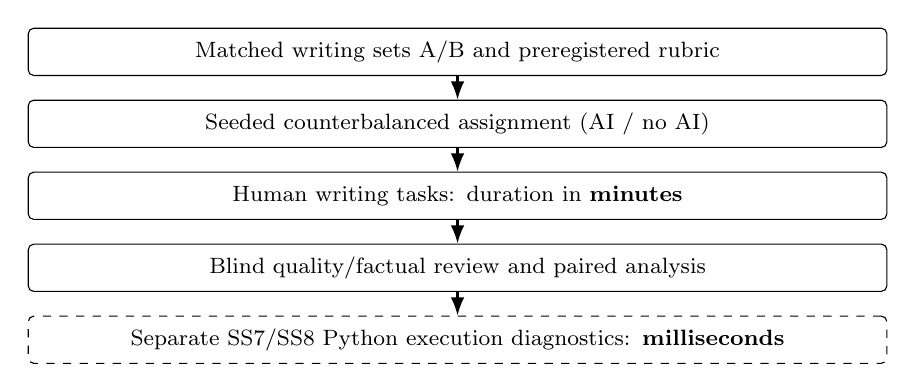
\begin{tikzpicture}[
    box/.style={draw,rounded corners=2pt,align=center,text width=0.88\columnwidth,minimum height=6mm,font=\footnotesize},
    arrow/.style={-Latex,thick},
    node distance=3mm
  ]
    \node[box] (tasks) {Matched writing sets A/B and preregistered rubric};
    \node[box,below=of tasks] (assignment) {Seeded counterbalanced assignment (AI / no AI)};
    \node[box,below=of assignment] (study) {Human writing tasks: duration in \textbf{minutes}};
    \node[box,below=of study] (scoring) {Blind quality/factual review and paired analysis};
    \node[box,below=of scoring,dashed] (engineering) {Separate SS7/SS8 Python execution diagnostics: \textbf{milliseconds}};
    \draw[arrow] (tasks)--(assignment);
    \draw[arrow] (assignment)--(study);
    \draw[arrow] (study)--(scoring);
    \draw[arrow,dashed] (scoring)--(engineering);
  \end{tikzpicture}
  \caption{Proposed research and reproducibility workflow. The dashed technical stream benchmarks analysis software and cannot estimate AI effects on human writing.}
  \label{fig:pipeline}
\end{figure}

\begin{table}[t]
  \centering
  \caption{Proposed crossover parameters (not yet implemented with real participants).}
  \label{tab:design}
  \begin{tabular}{@{}ll@{}}
    \toprule
    Design element & Proposed setting \\
    \midrule
    Conditions & Human with / without GenAI \\
    Task sets & Matched A and B \\
    Task length & 180--220 words \\
    Anchor facts & Five per task \\
    Time cap & 30 min per task \\
    Quality scale & 0--100, two raters \\
    Bootstrap draws & $B=10{,}000$ (demonstration) \\
    Random seed & 42 (analysis demonstration) \\
    \bottomrule
  \end{tabular}
\end{table}

\subsection{Primary outcome and estimand}
Let $T_{i,0}$ and $T_{i,1}$ be participant $i$'s completed writing time without and with AI, respectively, both in \emph{minutes}. The primary estimand is the population mean paired time saving, estimated by
\begin{equation}\label{eq:pairedtime}
  D_i=T_{i,0}-T_{i,1},\qquad
  \overline{D}=\frac{1}{n}\sum_{i=1}^{n}D_i.
\end{equation}
Here $D_i>0$ indicates time saved. The primary null is no mean benefit ($\mathbb{E}[D_i]\leq 0$), against a one-sided improvement alternative ($\mathbb{E}[D_i]>0$). This is equivalent to a negative difference when defining with-AI minus without-AI time. A paired bootstrap resamples \emph{participants}, preserving both observations within each pair. A 95\% percentile confidence interval provides descriptive uncertainty; a future confirmatory hypothesis test and analysis plan must specify directional testing, exclusions, and adequate sample size before data collection.

\subsection{Secondary outcomes and quality guardrail}
Two independent, blinded assessors score each response against accuracy/completeness (30 points), clarity (25), relevance (25), and professional language (20). Let $Q_{i,1}-Q_{i,0}$ be the with-AI minus without-AI quality difference. The provisional non-inferiority margin is $-5$ points; a formal claim would require a justified margin and the \emph{lower} confidence bound for the paired mean quality difference to exceed $-5$, rather than simply checking the point estimate.

Required-fact recall is the fraction of five anchor facts represented correctly. For all assessable factual claims, precision and F1 are
\begin{equation}\label{eq:factmetrics}
  P=\frac{C_s}{C_s+C_u},\quad
  R=\frac{A_c}{A_t},\quad
  F_1=\frac{2PR}{P+R},
\end{equation}
where $C_s$ and $C_u$ are supported and unsupported factual claims and $A_c/A_t$ is correct-anchor-fact coverage. Undefined-denominator cases are recorded as missing, not silently set to perfect scores. Reviewer disagreements and claim-annotation rules must be resolved in a pilot.

\subsection{Reproducibility, ethics, and software benchmark}
The public repository contains protocols, synthetic CSV records, Python validation and processing, unit tests, pinned dependencies, Docker support, and GitHub Actions. Participants have \emph{not} been recruited. In a future real study, obtain informed consent, record anonymized assignment and timing information, limit access to confidential drafts, and avoid publishing identifiable writing samples.

In a distinct educational engineering exercise, 5 warm-up runs and 100 measured executions benchmark the Python analysis pipeline on synthetic input sizes of 8, 16, and 32 rows. These timings are measured in \emph{milliseconds}, never pooled with the human-writing values in Eq.~\eqref{eq:pairedtime}. Failed executions remain in the failure-rate denominator; successful-run durations are summarized with median, p95/p99, IQR flags, and exploratory bootstrap intervals. No HTTP requests, chatbot latency, or requests-per-second performance are measured.

\section{Synthetic Demonstration Results}\label{sec:demonstration}
\textbf{All numbers in this section are generated demonstration data, not observations from recruited employees.} The paired CSV has four fictional participants with eight completed task records. The values in Table~\ref{tab:writing} reproduce the project's committed processed summary. Mean paired time saved was 3.875 min (95\% paired percentile-bootstrap interval [0.00, 6.25] min; 10,000 resamples, seed 42). This interval includes zero, and the sample is fictional; no effectiveness inference is justified.

\begin{table}[t]
  \centering
  \caption{SYNTHETIC writing-task demonstration: four fictional participants per condition. Values are mean $\pm$ sample SD.}
  \label{tab:writing}
  \begin{tabular}{@{}lrr@{}}
    \toprule
    Measure & No AI & With AI \\
    \midrule
    Time (min) & $23.38\pm2.56$ & $19.50\pm2.38$ \\
    Quality (0--100) & $81.63\pm4.82$ & $84.50\pm2.65$ \\
    Anchor recall (\%) & $85.00$ & $95.00$ \\
    \bottomrule
  \end{tabular}
\end{table}

Table~\ref{tab:software} summarizes a \emph{separate synthetic software log}, measured in milliseconds on the development system. It includes 100 timed Python executions after 5 warm-ups; all 100 completed, and 11 within-profile IQR flags were retained. These runs are \emph{not} 100 participants or AI treatment observations.

\begin{table}[t]
  \centering
  \caption{SYNTHETIC Python software benchmark (100 measured runs, milliseconds).}
  \label{tab:software}
  \begin{tabular}{@{}lr@{}}
    \toprule
    Statistic & Result \\
    \midrule
    Mean $\pm$ SD (ms) & $24.06\pm3.30$ \\
    Median (ms) & $22.94$ \\
    p95 / p99 (ms) & $31.27$ / $35.74$ \\
    Failures / IQR flags & $0$ / $11$ \\
    \bottomrule
  \end{tabular}
\end{table}

\section{Discussion and Limitations}\label{sec:discussion}
This report documents a proposed crossover experiment and reproducibility infrastructure. The synthetic writing comparison validates formulas and figure/table generation, but it cannot establish that GenAI improves employee productivity, maintains quality, or changes occupational outcomes. With four fictitious pairs, the interval cannot be treated as population evidence. Quality non-inferiority is also \emph{not} established: the observed demonstration quality difference is not a confidence-interval test.

The future study requires pilot-tested matched tasks, justified recruitment and power planning, control of task-order and learning effects, blinded reviewer training, prespecified exclusion rules, and an analysis that respects pairing. Uncertainty in the separate repeated-run software benchmark may be affected by machine-specific correlations; its measurements quantify software execution only, not writer speed. Reproducibility files and an audit trail are maintained in the accompanying repository. Upon collecting consented real data, the team will replace demonstration tables, transparently report deviations, and reassess the scientific conclusions.

\bibliographystyle{IEEEtran}
\bibliography{references}
\end{document}
